% Podstawowe definicje dla wszystkich dokumentów

\documentclass[11pt]{mwart}
%\setlength{\textwidth}{83pt}

\usepackage[OT4,plmath]{polski}
\usepackage{amsmath,amssymb,amsfonts,amsthm,mathtools}
\usepackage{color}
\usepackage{fontspec}
\usepackage{listings,times}

\usepackage{bbm}
\usepackage[colorlinks=true, urlcolor=blue]{hyperref}
\usepackage{url}
\usepackage{graphicx}

\graphicspath{{images/}}

\newcommand{\HRule}{\rule{\linewidth}{0.5mm}}

\newcommand{\term}[1]{
  \indent\textbf{#1}
  \vspace{5pt}
}

\usepackage{multicol}

\usepackage{lmodern} \normalfont
%\DeclareFontShape{EU1}{ptm}{bx}{n} { <-> ssub * cmr/bx/n }{}
%\DeclareFontShape{EU1}{ptm}{m}{sc} { <-> ssub * cmr/m/sc }{}

\usepackage{titletoc}

%\titlecontents{section}[3.8em]{}{\contentslabel{2.3em}}{\hspace*{-2.3em}}{\titlerule*[0.25pc]{ .}\contentspage}{}

\usepackage{fancyhdr}
\pagestyle{fancy}
\lhead[\fancyplain{Projekt Iron Coach - \doctitle}{Projekt Iron Coach - \doctitle}]         
    {\fancyplain{Projekt Iron Coach - \doctitle}{Projekt Iron Coach - \doctitle}}
\lfoot[\fancyplain{Studencka Pracownia Inżynierii Oprogramowania}{Studencka Pracownia Inżynierii Oprogramowania}]                 
    {\fancyplain{Studencka Pracownia Inżynierii Oprogramowania}{Studencka Pracownia Inżynierii Oprogramowania}}
\cfoot[\fancyplain{}{}] {\fancyplain{}{}}
\rfoot[\fancyplain{\thepage} {\thepage}]  {\fancyplain{\thepage}{\thepage}}


%\pagestyle{myheadings}
%\markright{Projekt Iron Coach \hfill \doctitle \hfill \rightmark}


\newcommand{\titlep}[2] {
  \newcommand{\doctitle}{#1}
  \begin{titlepage}
    \begin{center}
      \textsc{\large Studencka Pracownia Inżynierii Oprogramowania}\\
      \textsc{\LARGE Uniwersytet Wrocławski \\Instytut Informatyki}\\[1.5cm]


      \vspace{3cm}

      % Author and supervisor
      \begin{minipage}{\textwidth}
        \begin{center} \Large
          Łukasz \textsc{Czapliński},
          Diana \textsc{Czepirska},
          Artur \textsc{Jarocki}
        \end{center}
      \end{minipage}

      \vspace{0.5cm}



      % Title
      \HRule \\[0.4cm]
      { \Huge \bfseries Iron Coach  \\[1cm] }

      \textsc{\Large #1\\\large Wersja #2}\\[0.5cm]

      \HRule \\[1.5cm]

      \vspace{1cm}

      
\includegraphics[width=0.15\textwidth]{non-starred.png}~\\[1cm]
      
      \vfill
      

      \vspace{1cm}

      % Bottom of the page
      {\large Wrocław 2013}

    \end{center}
  \end{titlepage}
  \clearpage
}

\newcommand{\chist}[1]{
  {\large{Historia zmian}} \\ \vspace{1cm}
  \begin{tabular}{r | l | l}
    Wersja & Opis & Autor \\ 
    \hline
    \noalign{\smallskip}
    #1
  \end{tabular}
}

\begin{document}
\titlep{Harmonogram}{1.3}
\chist{ 1.0 & 2013-11-01 & Powstanie szkieletu dokumentu & Łukasz Czapliński \\
				1.1 & 2013-11-05 & Dodanie wykresu Gantta & Diana Czepirska \\
				1.2 & 2013-11-26 & Dodanie opisu etapów & Diana Czepirska \\
        1.3 & 2013-11-28 & Poprawki stylistyczne & Diana Czepirska \\
}
\tableofcontents
\clearpage
\newcommand{\tabb}{\begin{tabular}{l p{8cm}}}
%\renewcommand{\sectionmark}[1]{}
\renewcommand{\subsectionmark}[1]{}
\section{Wstęp}
	Proces budowy aplikacji Iron Coach został podzieony na 14 etapów w celu lepszej organizacji pracy. Przy pisaniu systemu będzie pracowało trzech specjalistów, każdy z nich będzie pracował 8 godzin dziennie, 5 dni w tygodniu - korzystając z tego założenia został oszacowany czas trwania każdego etapu budowy programu Iron Coach. Łączny czas budowy aplikacji szacowany jest na 6 (do 7) miesięcy.
	W kolejnych sekcjach znajdują się opisy każdego z etapów wraz z datami ich rozpoczęcia i zakończenia, a także graficzna prezentacja harmonogramu (w formie wykresu Gantta).
\section{Opis kolejnych stadiów}
\subsection{Znajdowanie potrzeb, zbieranie wymagań}
	\tabb
		\textbf{Data rozpoczęcia:} & 01-12-2013\\
		\textbf{Data zakończenia:} & 10-12-2013\\
		\textbf{Czas trwania:} & 7 dni\\
		\textbf{Opis:} & Etap ten polega na obserwacji ludzi (potencjalnych użytkowników aplikacji Iron Coach) w celu uzyskania informacji o ich problemach, potrzebach i wymaganiach związanych z treningami (szczególnie bieganiem) oraz na analizie zebranych informacji i wyciągnięciu wniosków dotyczących tego, co powinno się znaleźć w aplikacji Iron Coach.
	\end{tabular}
\subsection{Zaprojektowanie interfejsu użytkownika}
	\tabb
		\textbf{Data rozpoczęcia:} & 11-12-2013\\
		\textbf{Data zakończenia:} & 13-12-2013\\
		\textbf{Czas trwania:} & 3 dni\\
		\textbf{Opis:} & Etap projektowania interfejsu użytkownika polega na wymyśleniu i zaprojektowaniu wstępnego interfejsu, na podstawie którego stworzony zostanie pierwszy prototyp.
	\end{tabular}
\subsection{Opracowanie prototypu rozwiązania}
	\tabb
		\textbf{Data rozpoczęcia:} & 16-12-2013\\
		\textbf{Data zakończenia:} & 19-12-2013\\
		\textbf{Czas trwania:} & 4 dni\\
		\textbf{Opis:} & Etap ten polega na zbudowaniu pierwszego prototypu w celu przedstawienia użytkownikom jak może wyglądać aplikacja Iron Coach.
	\end{tabular}
\subsection{Ocena prototypu, uściślenie wymagań na jej podstawie}
	\tabb
		\textbf{Data rozpoczęcia:} & 20-12-2013\\
		\textbf{Data zakończenia:} & 02-01-2014\\
		\textbf{Czas trwania:} & 10 dni\\
		\textbf{Opis:} & Ten etap składa się z przekazania prototypu do wypróbowania użytkownikom, zebrania ich uwag oraz z uściślenia wymagań na podstawie zebranych informacji.
	\end{tabular}
\subsection{Poprawa interfejsu}
	\tabb
		\textbf{Data rozpoczęcia:} & 03-01-2014\\
		\textbf{Data zakończenia:} & 13-01-2014\\
		\textbf{Czas trwania:} & 7 dni\\
		\textbf{Opis:} & Poprawa interfejsu polega na ponownym zaprojektowaniu interfejsu użytkownika zgodnie z wymaganiami ustalonymi w poprzednim etapie.
	\end{tabular}
\subsection{Projekt i wykonanie bazy danych}
	\tabb
		\textbf{Data rozpoczęcia:} & 03-01-2014\\
		\textbf{Data zakończenia:} & 08-01-2014\\
		\textbf{Czas trwania:} & 4 dni\\
		\textbf{Opis:} & Etap ten polega na zaprojektowaniu bazy danych, z której będzie korzystał Iron Coach oraz wykonaniu jej.
	\end{tabular}
\subsection{Napisanie rdzenia aplikacji}
	\tabb
		\textbf{Data rozpoczęcia:} & 03-01-2014\\
		\textbf{Data zakończenia:} & 06-03-2014\\
		\textbf{Czas trwania:} & 45 dni\\
		\textbf{Opis:} & Etap ten polega na implementacji aplikacji Iron Coach.
	\end{tabular}
\subsection{Testy wewnętrzne}
	\tabb
		\textbf{Data rozpoczęcia:} & 07-03-2014\\
		\textbf{Data zakończenia:} & 17-03-2014\\
		\textbf{Czas trwania:} & 7 dni\\
		\textbf{Opis:} & Etap ten polega na przeprowadzeniu testów oprogramowania mających na celu wyszukanie błędów w kodzie, sprawdzenie zgodności ze specyfikacją itd.
	\end{tabular}
\subsection{Naprawa wykrytych błędów}
	\tabb
		\textbf{Data rozpoczęcia:} & 18-03-2014\\
		\textbf{Data zakończenia:} & 26-03-2014\\
		\textbf{Czas trwania:} & 7 dni\\
		\textbf{Opis:} & Etap ten polega na naprawie błędów wykrytych w poprzednim etapie.
	\end{tabular}
\subsection{Testowanie z udziałem użytkowników, analiza uwag}
	\tabb
		\textbf{Data rozpoczęcia:} & 27-03-2014\\
		\textbf{Data zakończenia:} & 16-04-2014\\
		\textbf{Czas trwania:} & 21 dni\\
		\textbf{Opis:} & Etap ten polega na przetestowaniu aplikacji Iron Coach przez przedstawicieli grupy ludzi, dla których jest budowana, co ma na celu sprawdzenie zgodności tej aplikacji z oczekiwaniami użytkowników.
	\end{tabular}
\subsection{Poprawa błędów}
	\tabb
		\textbf{Data rozpoczęcia:} & 17-04-2014\\
		\textbf{Data zakończenia:} & 30-04-2014\\
		\textbf{Czas trwania:} & 14 dni\\
		\textbf{Opis:} & Etap ten polega na poprawie błędów wykrytych w poprzednich etapach. 
	\end{tabular}
\subsection{Dodanie nowych funkcji}
	\tabb
		\textbf{Data rozpoczęcia:} & 01-05-2014\\
		\textbf{Data zakończenia:} & 09-05-2014\\
		\textbf{Czas trwania:} & 7 dni\\
		\textbf{Opis:} & Etap ten ma na celu dodanie do projektu Iron Coach funkcji, których brak (i potrzebę ich implementacji) stwierdzono np. w testach z użytkownikami.
	\end{tabular}
\subsection{Ponowne testy}
	\tabb
		\textbf{Data rozpoczęcia:} & 12-05-2014\\
		\textbf{Data zakończenia:} & 23-05-2014\\
		\textbf{Czas trwania:} & 10 dni\\
		\textbf{Opis:} & Jeśli w dwóch poprzednich etapach zostały dokonane jakieś zmiany, w tym etapie powinny zostać powtórzone wszystikie testy (zarówno te związane z samym kodem aplikacji, jak i testy z udziałem użytkowników).
	\end{tabular}
\subsection{Ostateczne poprawki}
	\tabb
		\textbf{Data rozpoczęcia:} & 26-05-2014\\
		\textbf{Data zakończenia:} & 06-06-2014\\
		\textbf{Czas trwania:} & 10 dni\\
		\textbf{Opis:} & Dokonanie ostatecznych poprawek błędów wykrytych w poprzednim etapie.
	\end{tabular}

\section{Wykres Gantta}
  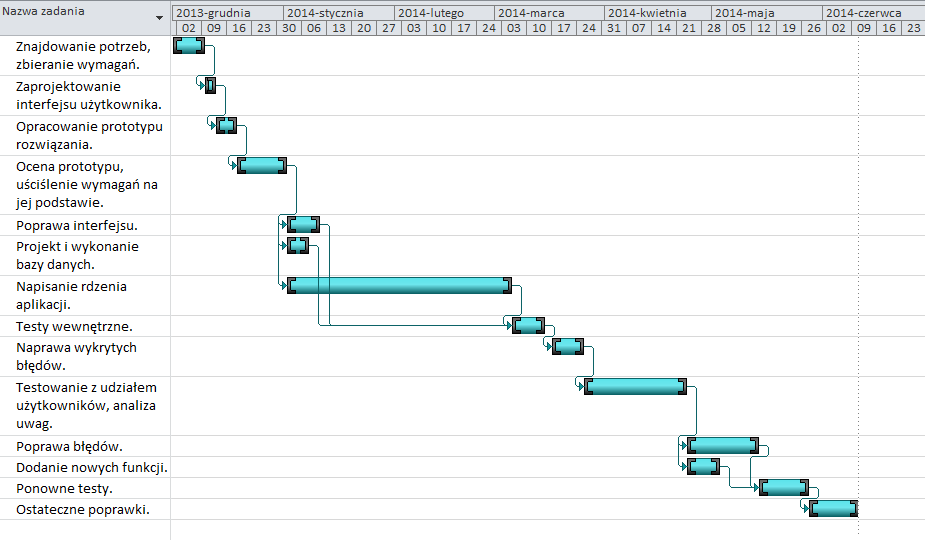
\includegraphics[angle=270]{wykres_gantta2.png}
\end{document}
